\documentclass{jarticle}

\usepackage{twocolumn}
% \usepackage[dvi ps]{graphicx}%%画像を読み込む
\usepackage[dvipdfmx]{graphicx}
\usepackage{subfigure}
\usepackage{amsmath}          %%genfrac http://www.biwako.shiga-u.ac.jp/sensei/kumazawa/tex/form006.html
\usepackage{ulem}             %%http://biwako.shiga-u.ac.jp/sensei/kumazawa/tex/ulem.html     uline,uuline,uwave,sout,xoutなど
\usepackage{multirow}
\usepackage{here}
% \usepackage{setspace}
\usepackage{chukan2018}       %%最後に読み込むこと!(最後に読み込まないと\textwidthなどの設定が反映されない)

\pagestyle{empty} %ページ番号を入れるときにはコメントアウトする

\begin{document}

\linesparpage{50}

\title{
カニ模倣型ロボットの開発に向けた細径空圧筋の改良
}
\etitle{
Improvement of Thin Pneumatic Muscles for Development of Crab-type Robot
}
\author{
研究者 濱口 紘生  指導教員  中西 大輔
}
\eauthor{
Keywords: McKibben Pneumatic Actuater, Exoskeleton, Biomimetic Robot
}

\maketitle

\thispagestyle{empty}  %1ページ目にページ番号を入れるときにはコメントアウトする

%%%%%%%%%%%%%%%%%%%%%%%%%%%%%%%%%%%%%%%%%%%%%%%%%%%%%%%%%%%%%%%%%%%%%%%%%%%%%%%
\section{緒言}

代表的な人工筋肉として,圧縮空気を印加することにより骨格筋のように収縮するMcKibben型人工筋肉(MPA)があげられる.
従来は直径が数十mm程度のものが多かったが,近年では数mm程度のMPAが注目を集めている\cite{wakimoto}.
その細さを活かして小さい筋肉,あるいは集積によって複雑な筋肉を表現可能なことから,筋骨格系ロボットに盛んに用いられている\cite{wakimoto}.
一方で,甲殻類のような外骨格を有する生物模倣ロボットでは,アクチュエータの配置が困難なことからワイヤ駆動や関節にサーボモータを配置したものが主流であった\cite{crabrobot1}.
細径MPAであれば骨格内部にアクチュエータを配置することが可能であり,実際の生物に近い構成でロボットを作成することが可能である.そこで本研究では外骨格生物のうち甲殻類の蟹をモデルに,
実際の蟹の筋肉と関節の構造を参考にして細径MPAを使用した蟹の歩脚ロボットの開発に取り組む.

%%%%%%%%%%%%%%%%%%%%%%%%%%%%%%%%%%%%%%%%%%%%%%%%%%%%%%%%%%%%%%%%%%%%%%%%%%%%%%%
\vspace*{-2mm}
\section{MPAおよび羽状筋について}

従来のMPAと細径MPAを図\ref{fig:MPA}に示す.通常のMPA(図\ref{fig:MPA}左)と比べて細径MPA(図\ref{fig:MPA}中,右)は細くて軽量のため狭いスペースへの配置と集積が可能である.
また複数の細径MPAを集積することで複雑な筋肉の再現が可能である.
また先行研究\cite{crabrobot2}で開発されたロボットに搭載された細径MPAを用いた羽状筋を図\ref{fig:crabrobot}に示す.
羽状筋とは羽のように筋繊維が斜めに並んだ筋肉である.
先行研究\cite{crabrobot2}ではこの羽状筋を用いてカニの歩脚を模した外骨格型ロボットを開発し,脚の開閉動作の実現に成功した.
しかし羽状筋の構成方法や細径MPAの収縮性能などを原因として,実際の蟹と比べて可動域が狭いという課題が残された.
また細径MPAの制作過程の煩雑さも課題であった.
本研究ではまずこれらの課題を解決することで,より実際の蟹に近い構造や可動域を有するロボットの開発を目指す.

%%%%%%%%%%%%%%%%%%%%%%%%%%%%%%%%%%%%%%%%%%%%%%%%%%%%%%%%%%%%%%%%%%%%%%%%%%%%%%%
\vspace*{-2mm}
\section{細径MPAおよび羽状筋構造の改良}

まず細径MPAの制作方法の改良を行った.先行研究では図\ref{fig:OringMPA}上のように,MPAを構成するシリコンチューブとスリーブを端部で糸で縛り接着剤で固定する方式を採用していたが,
糸の締結に時間と練度を必要とすることや,度々空気漏れを生じるという難点があった.そこで本研究では端部部品を改良し,ゴムと端部を接着剤で,
スリーブと端部をOリングと接着剤でそれぞれ固定する方式へと変更した(図\ref{fig:OringMPA}下).これにより細径MPAに練度が不要となり,作成時間も大幅に短縮された.

\begin{figure}[H]
  \begin{minipage}[b]{0.47\columnwidth}
    \centering
    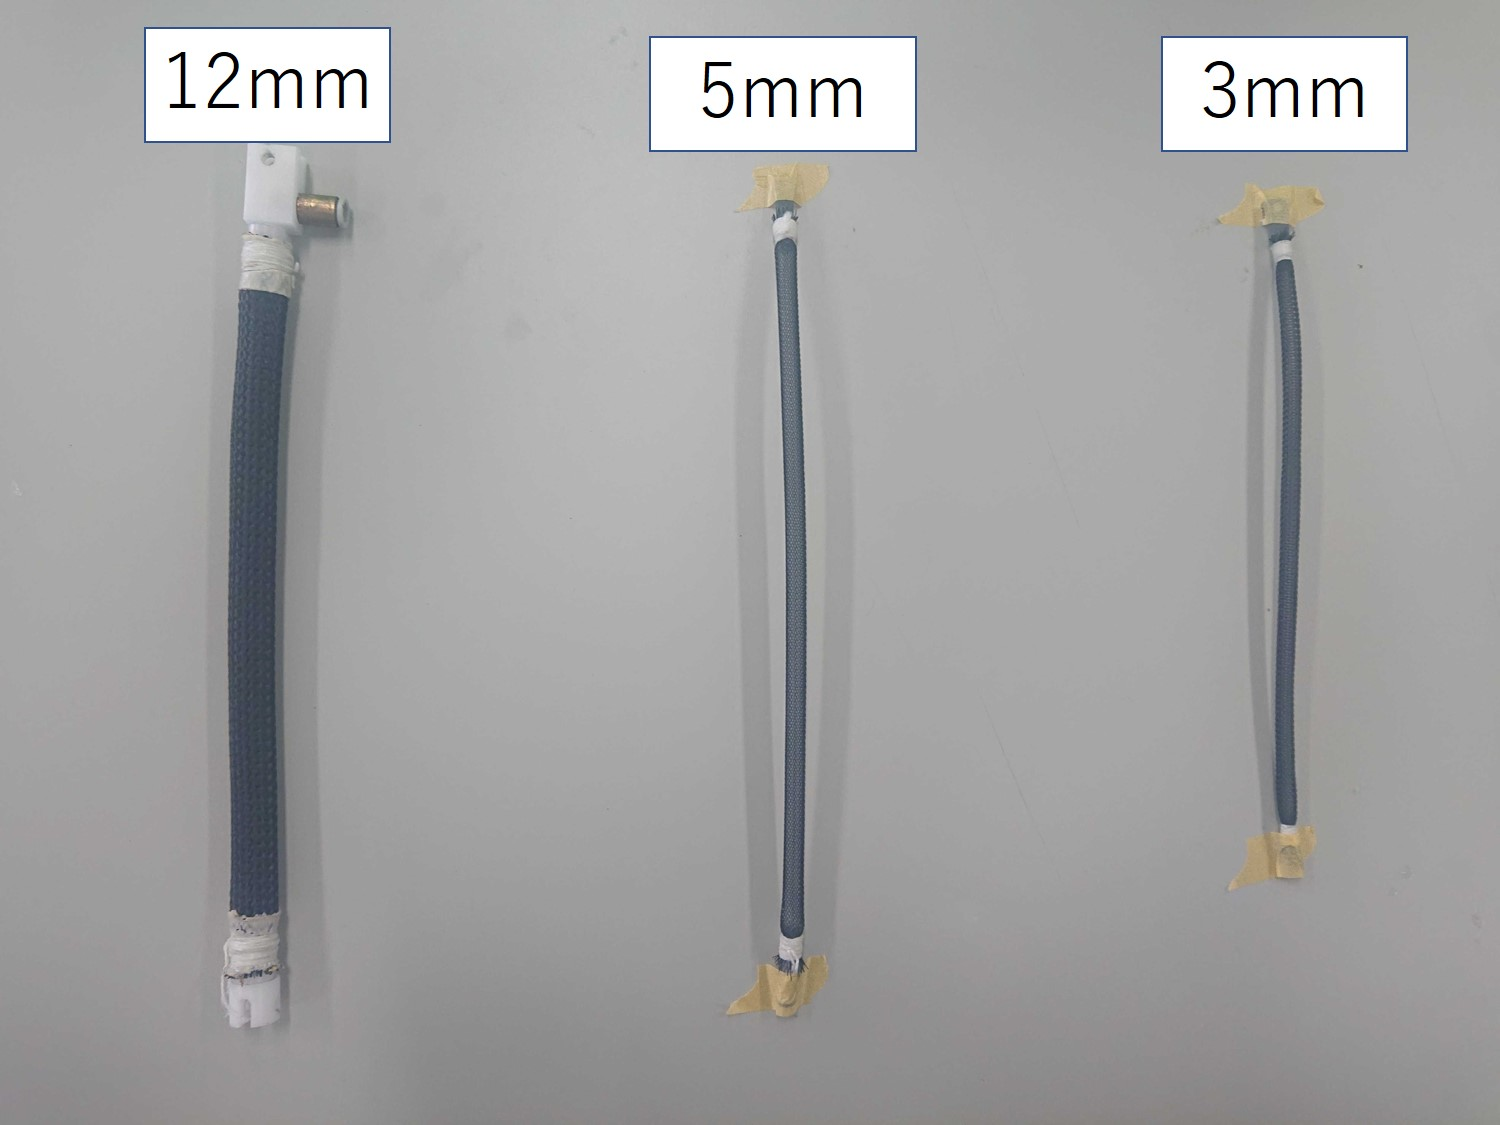
\includegraphics[scale=0.13]{image/mpa.JPG}
    \vspace{-4mm}
    \caption{MPAの外径}
    \label{fig:MPA}
  \end{minipage}
  \hspace{0.04\columnwidth}
  \begin{minipage}[b]{0.47\columnwidth}
    \centering
    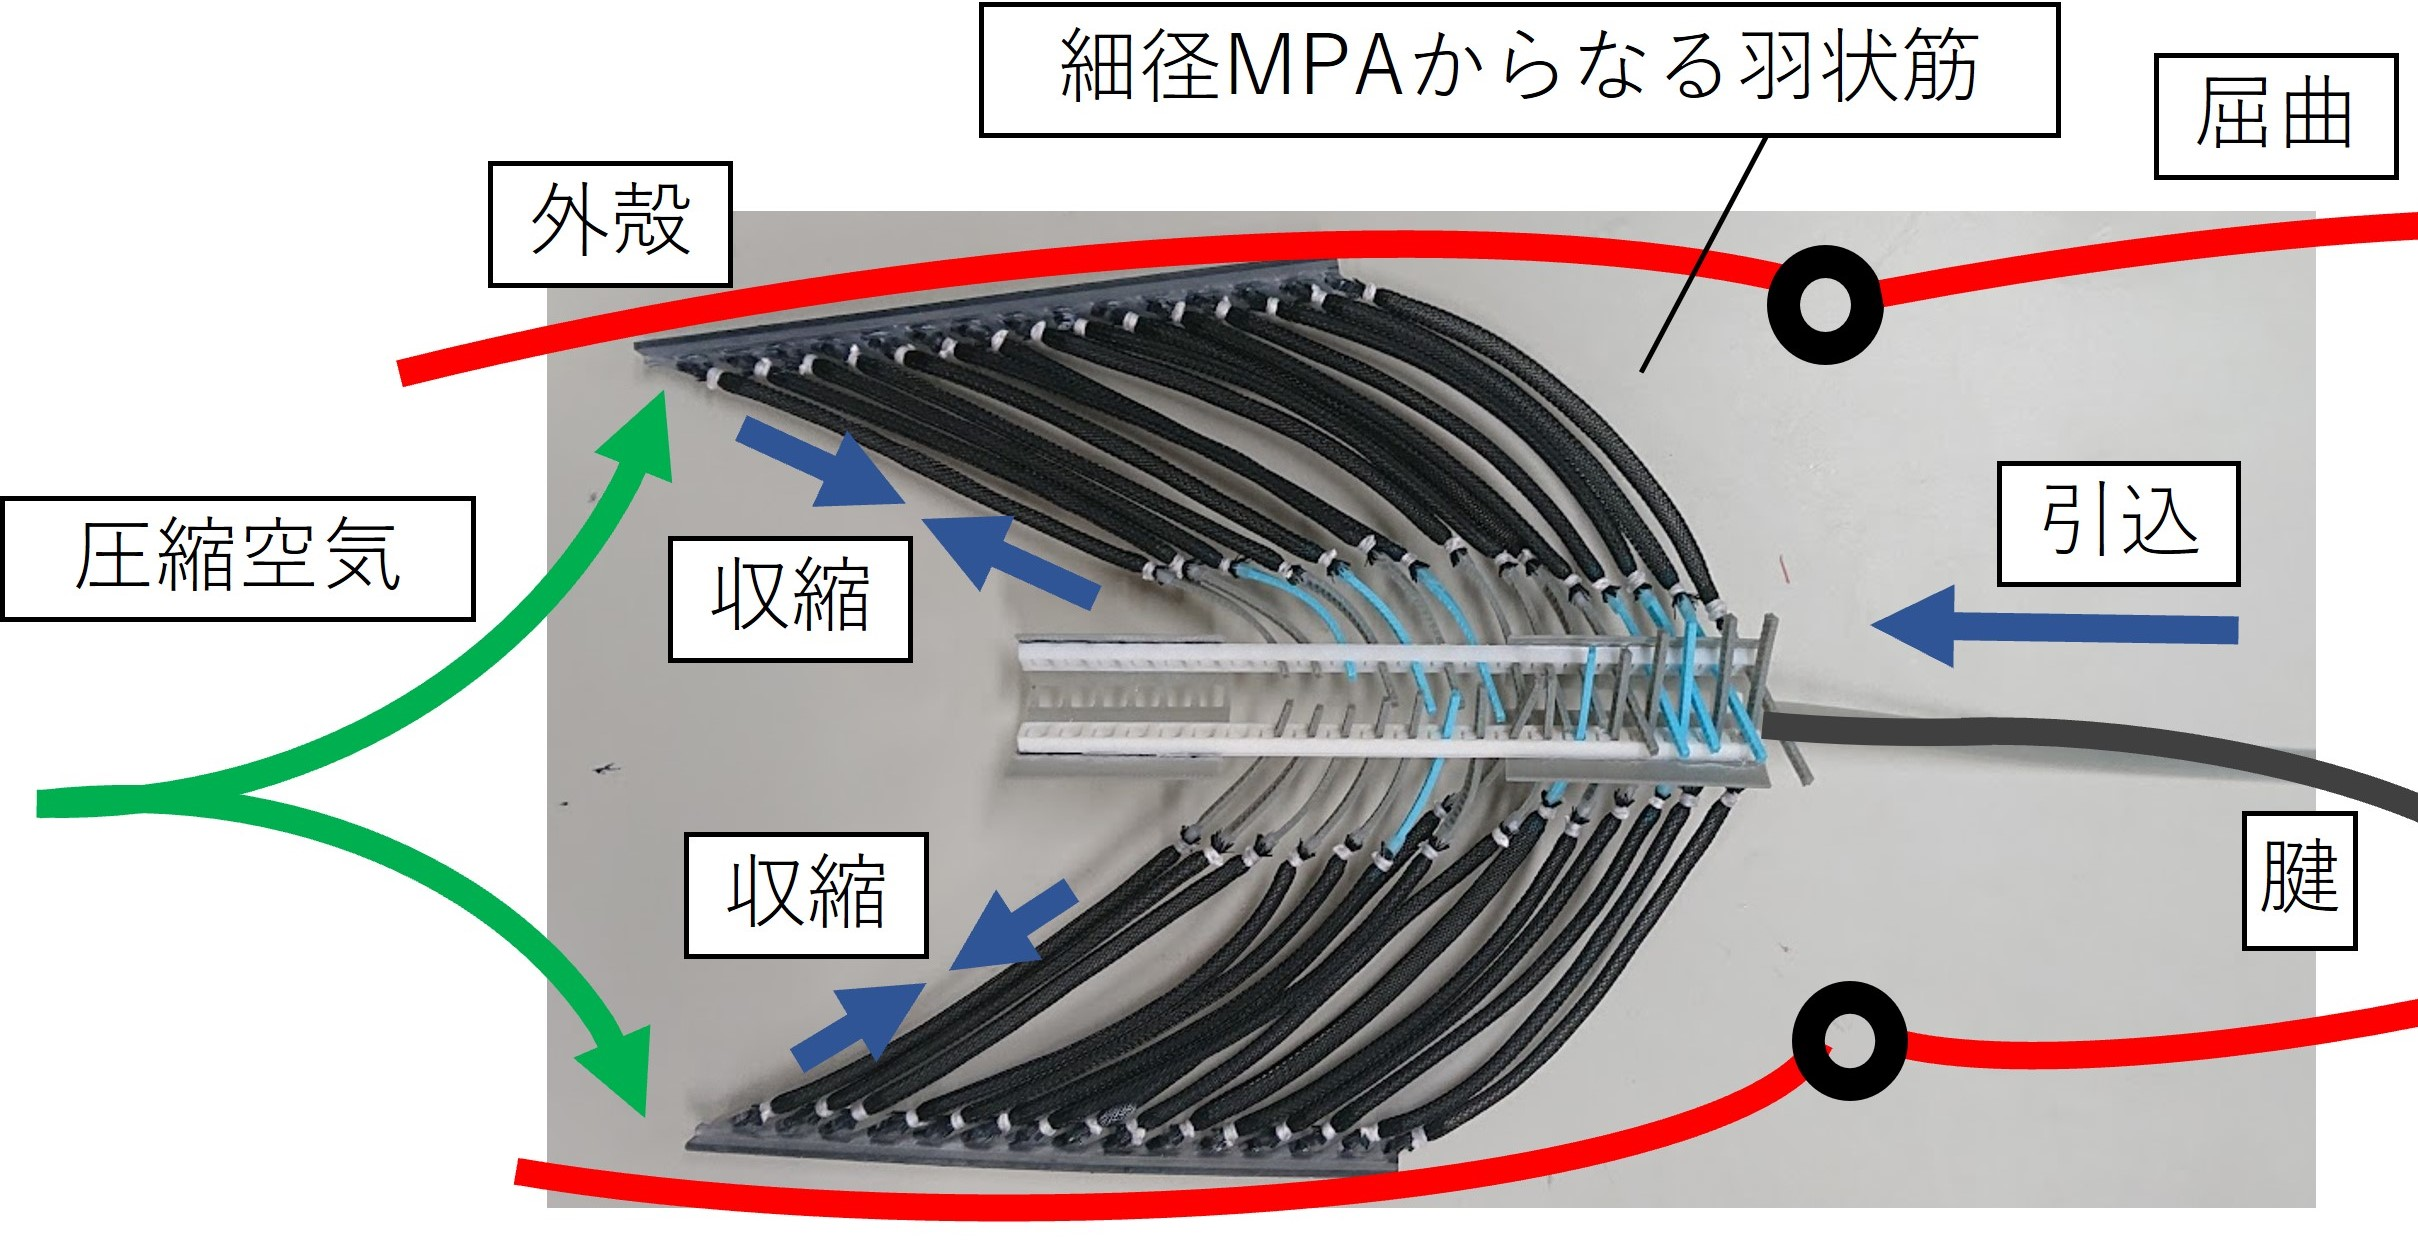
\includegraphics[scale=0.19]{image/mosiki.JPG}
    \vspace{-6mm}
    \caption{蟹模倣ロボット\cite{crabrobot2}}
    \label{fig:crabrobot}
  \end{minipage}
\end{figure}
\vspace*{-5mm}
\begin{figure}[H]
  \begin{minipage}[b]{0.47\columnwidth}
    \centering
    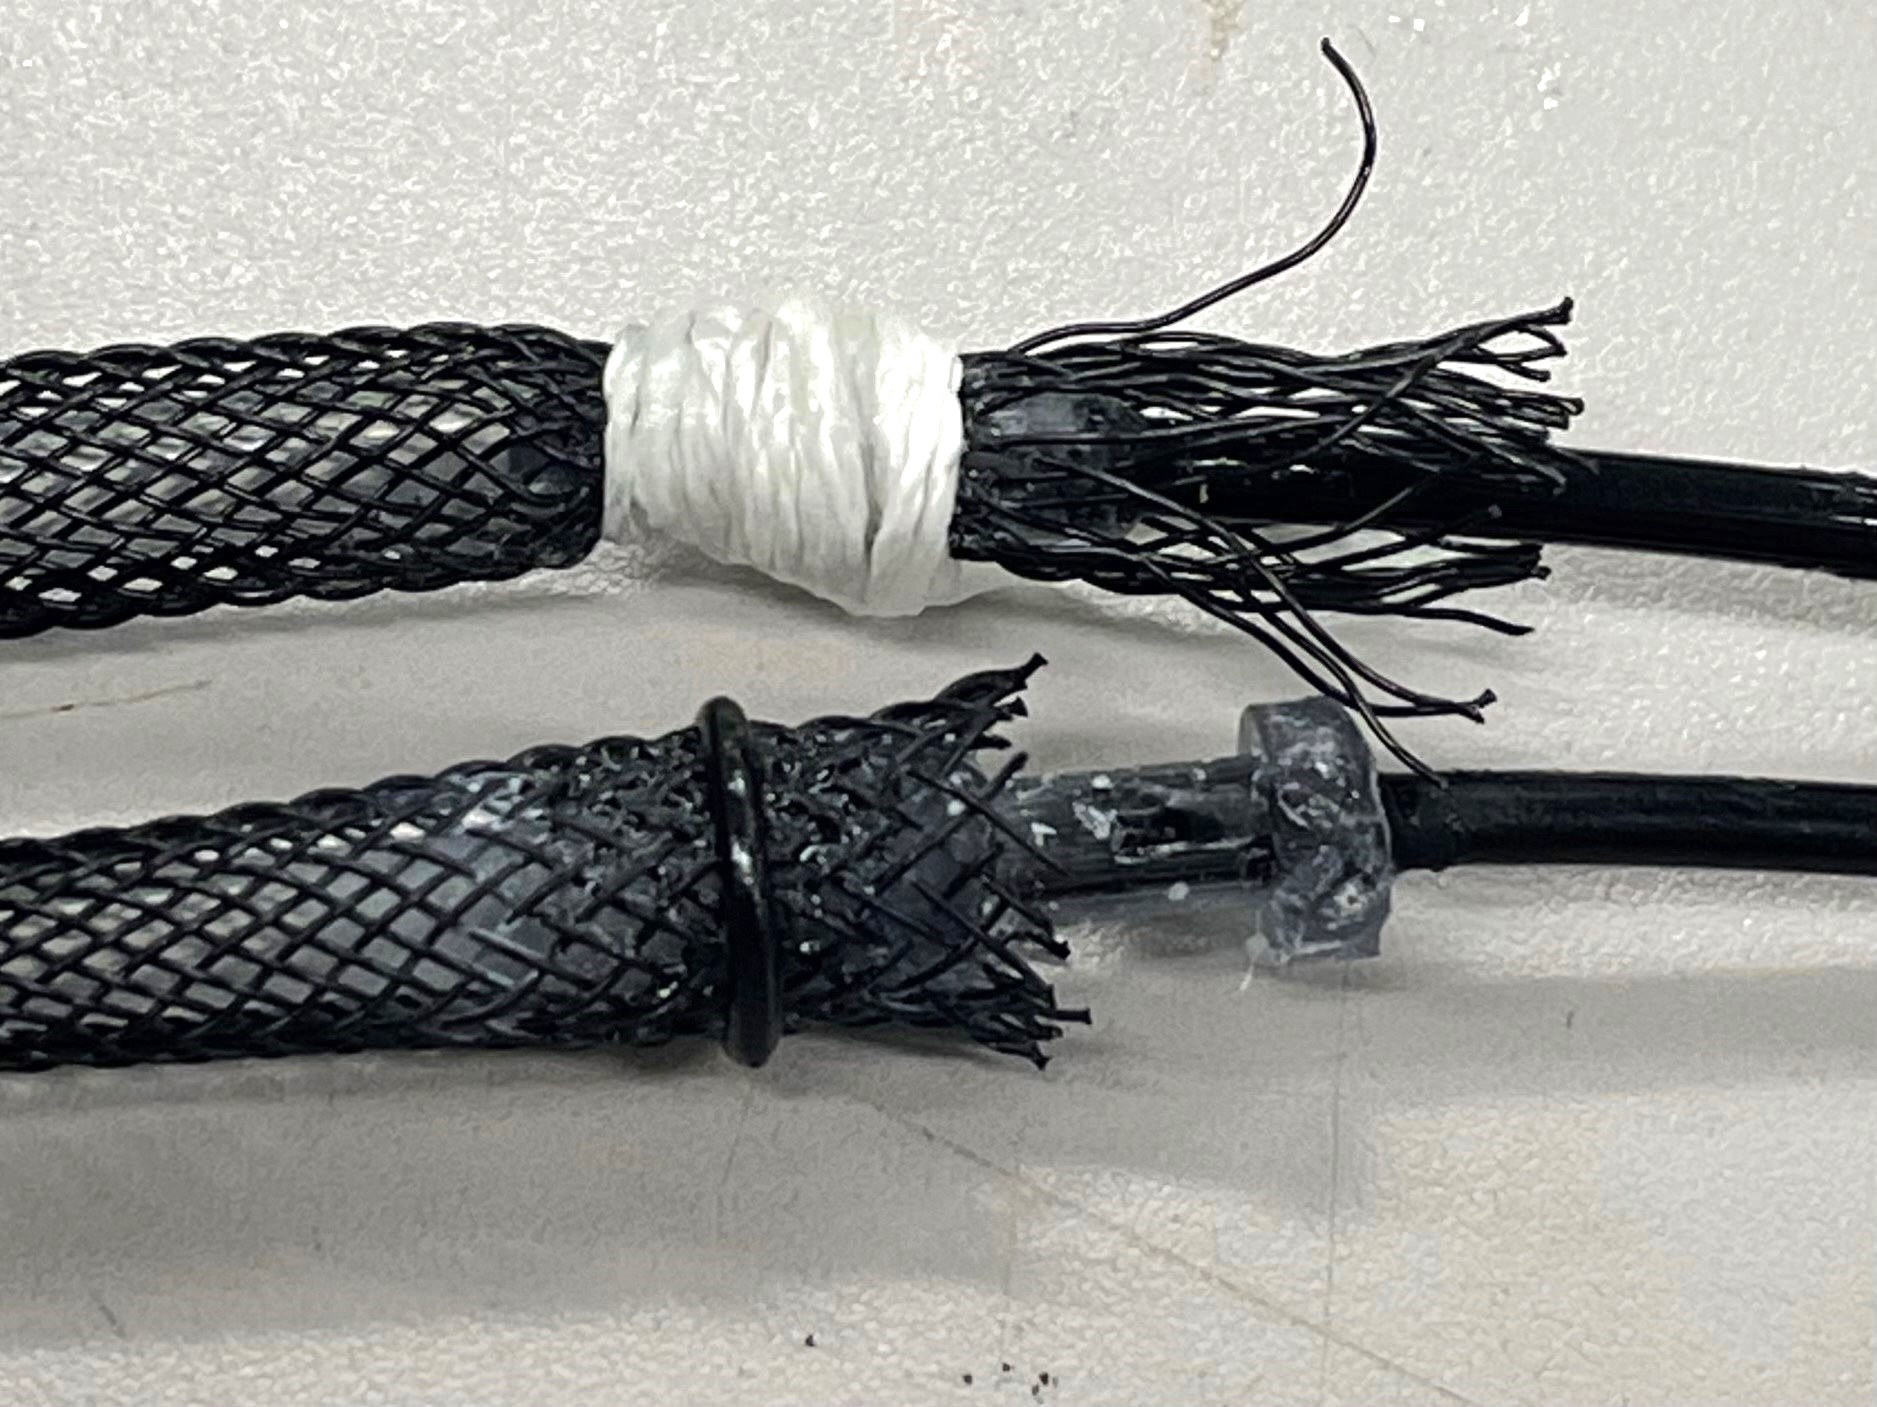
\includegraphics[scale=0.05]{image/mpa_oring_1.jpg}
    \vspace{-2mm}
    \caption{細径MPA締結方法}
    \label{fig:OringMPA}
  \end{minipage}
  \hspace{0.04\columnwidth}
  \begin{minipage}[b]{0.47\columnwidth}
    \centering
    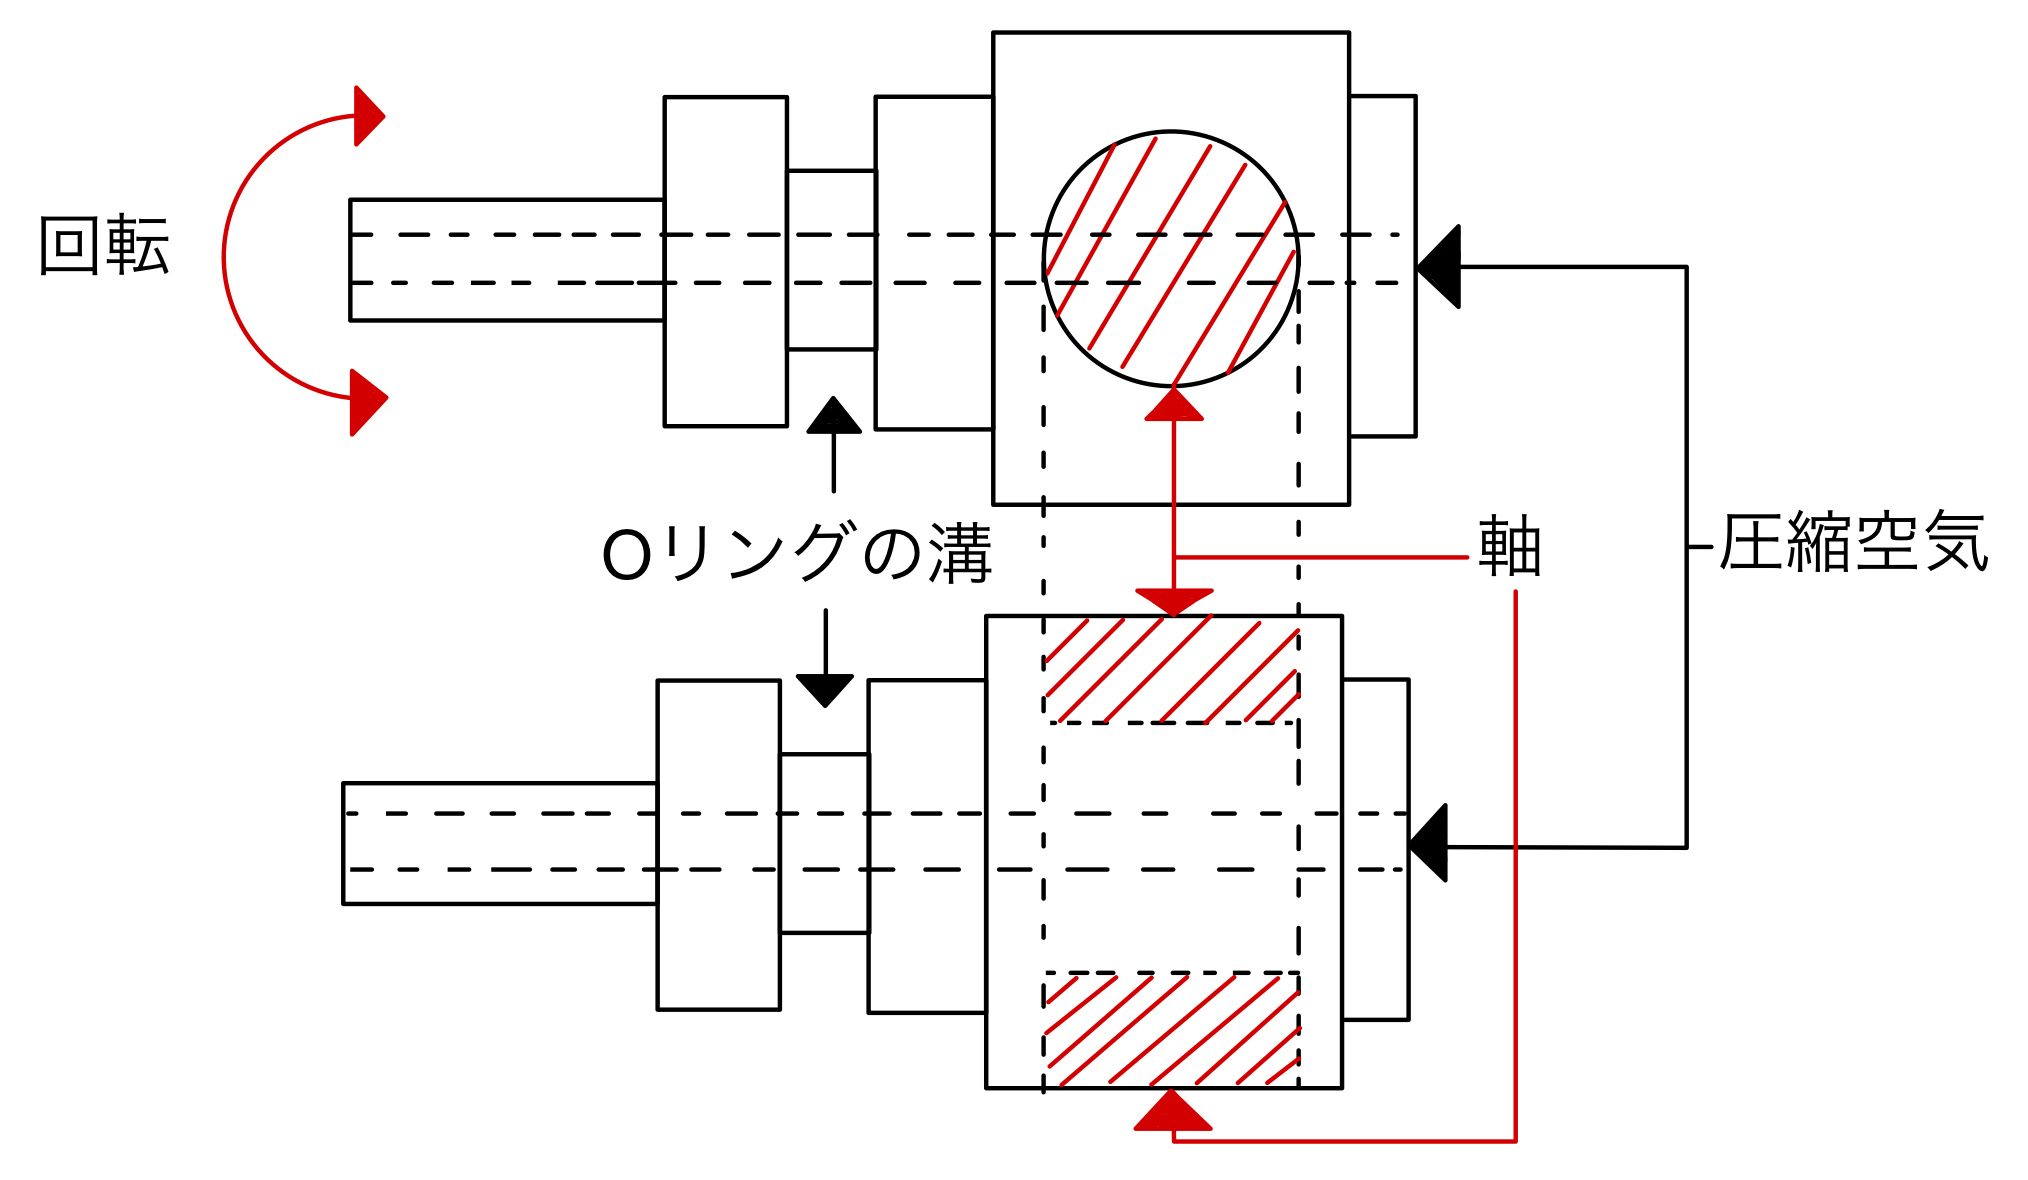
\includegraphics[scale=0.047]{image/MPA_irast.jpg}
    \vspace{-2mm}
    \caption{細径MPA端部部品}
    \label{fig:MPAparts}
  \end{minipage}
\end{figure}


続いて細径MPAの収縮性能向上に取り組んだ.
先行研究において開発された細径MPAにおいては,折癖の影響からスリーブが多少膨らんだ状態で作成されていたため,
圧力印加時の収縮量が減少してしまっていた.本研究ではメッシュの中に直径2mmの丸棒を差し込んで固定した状態でホットプレートで加熱することで熱可塑変化させた.
折癖をとるとともにスリーブの初期直径を2mmにまで小さくすることに成功し,収縮量を向上させることができた.


最後に,細径MPAを羽状配置するために端部の部品の構造を改良した.羽状筋は収縮した際に筋肉の角度が変化するが,先行研究(図\ref{fig:crabrobot})では
根元の角度が固定されており,腱の引き込みの妨げになっていた.そこで本研究では図\ref{fig:MPAparts}の細径MPAの端部の部品を作成した.
図\ref{fig:MPAparts}の赤い斜線部の穴を回転の軸にして細径MPAの角度を自由に変化することができ,これにより細径MPA動作時に端部の部品に干渉しないことが確認できた.
%%%%%%%%%%%%%%%%%%%%%%%%%%%%%%%%%%%%%%%%%%%%%%%%%%%%%%%%%%%%%%%%%%%%%%%%%%%%%%%
\vspace*{-2mm}
\section{実機の設計・作成方法}
\vspace*{-1mm}
\subsection{外骨格の設計について}
作成した実機を図\ref{fig:jikki}に示す.
今回の研究では甲殻類のうち蟹のズワイガニの歩脚モデルに機体を作成した.
機体作成時には先行研究\cite{crabrobot2}のズワイガニの歩脚の各部寸法と,本研究で新たに解剖した際に得られた可動域をもとにしてモデリングした.
ただし機体内部に細径MPAや腱部品などを配置する必要があるため,実測値に対して直径方向には7倍,長手方向には3.5倍のサイズとした.
可動域を実際の蟹に近づけるために腕節部だけ長手方向に6.3倍した.
作成にはMPA方式の3Dプリンタを使用し,関節部にはベアリングを入れている.
長手方向の具体的な寸法としては,長節が350 mm,腕節が256 mm,前節が245 mm,指節が100 mmである.
%%%%%%%%%%%%%%%%%%%%%%%%%%%%%%%%%%%%%%%%%%%%%%%%%%%%%%%%%%%%%%%%%%%%%%%%%%%%%%%
\subsection{細径MPAを用いた羽状筋の再現について}
蟹の外骨格内部の筋配置を図\ref{fig:kinhaichi}に示す.蟹の筋肉は外骨格から腱に向かって斜めに並んだ羽状筋となっている.
羽状筋は収縮した際,各筋繊維の角度が大きくなるだけで,膨張しないため狭い空間で働くのに適している.また,長節から腕節に配置されている羽状筋は節の回転軸によらず縦に格納されており,腱がねじれるようになっている.

本研究では,徐行きのような蟹の駆動機構を再現するため細径MPAを用いた羽状筋の開発を行った.開発した羽状筋を図\ref{fig:muscle}に示す.
上記で説明した羽状筋の筋繊維は1本ずつ長さが異なっているが,作成方法と関節の可動域の幾何学的計算を簡易化するため図\ref{fig:muscle}のように細径MPAの長さがすべて等しくなるように設計した.
図\ref{fig:muscle}の細径MPAの端部にある黒い部品は3章で紹介した細径MPAの収縮に合わせて角度が自由に変化でき,圧縮空気を各細径MPAへ一度に供給することができる部品である.
この部品は光造形方式の3Dプリンターで作製した.
また図\ref{fig:muscle}にある灰色の部品は蟹の腱を模したもので,TPU素材を使用してFDM方式の3Dプリンターで作製したので柔軟性が高くねじれに対応可能である.
腱と外骨格は全てねじで固定しており,腱の張り具合は可能な仕組みになっている.

可動域の幾何学的計算は図\ref{fig:keisan_1}のような簡易モデルをもとに三角関数などを用いて式(\ref{theta2}),(\ref{Se})を導いた.
収縮前の細径MPAの長さ$\ell_1$と細径MPAの付着点間の垂直距離をdを用いて収縮後の細径MPAと腱のなす角を$\theta_{2}$を計算した(式\ref{theta2}).
収縮前の細径MPAの長さ$\ell_1$,その時の細径MPAと腱のなす角$\theta_{1}$,収縮後の細径MPAの長さ$\ell_2$,その時の細径MPAと腱のなす角$\theta_{2}$を用いて誌細径MPAの収縮による腱の水平移動距離$S_e$を計算した(式\ref{Se}).
なお,細径MPAの収縮率は20%,$\theta_{1}$=20として計算を行った.
\begin{eqnarray}
	\label{theta2} \theta_2 &=& \sin^{-1}\left(\frac{d}{0.8 \ell_1}\right)\\
  \label{Se} S_e &=& \ell_1 \cos\theta_1 - \ell_2 \cos\theta_2
\end{eqnarray}
%%%%%%%%%%%%%%%%%%%%%%%%%%%%%%%%%%%%%%%%%%%%%%%%%%%%%%%%%%%%%%%%%%%%%%%%%%%%%%%
\vspace*{-2mm}
\section{動作実験}
長節から指節にかけてMPAを配置し動作実験を行った.関節の動きを確認しやすくするために長節-腕節間と前節-指節間は機体を寝かせた状態,腕節-前節間は機体を立てた状態で動作実験を行った.
また,初期位置は開筋か閉筋のどちらか一方が張った状態の位置にし,空気の印加は手動で0MPa~0.6MPaまで調整して動作させた.

長節-腕節間の動作結果を図\ref{fig:move1},腕節-前節の動作実験を図\ref{fig:move2},前節-指節の動作実験を図\ref{fig:move3}に示す.


\begin{figure}[t]
  \begin{minipage}[b]{0.47\columnwidth}
    \centering
    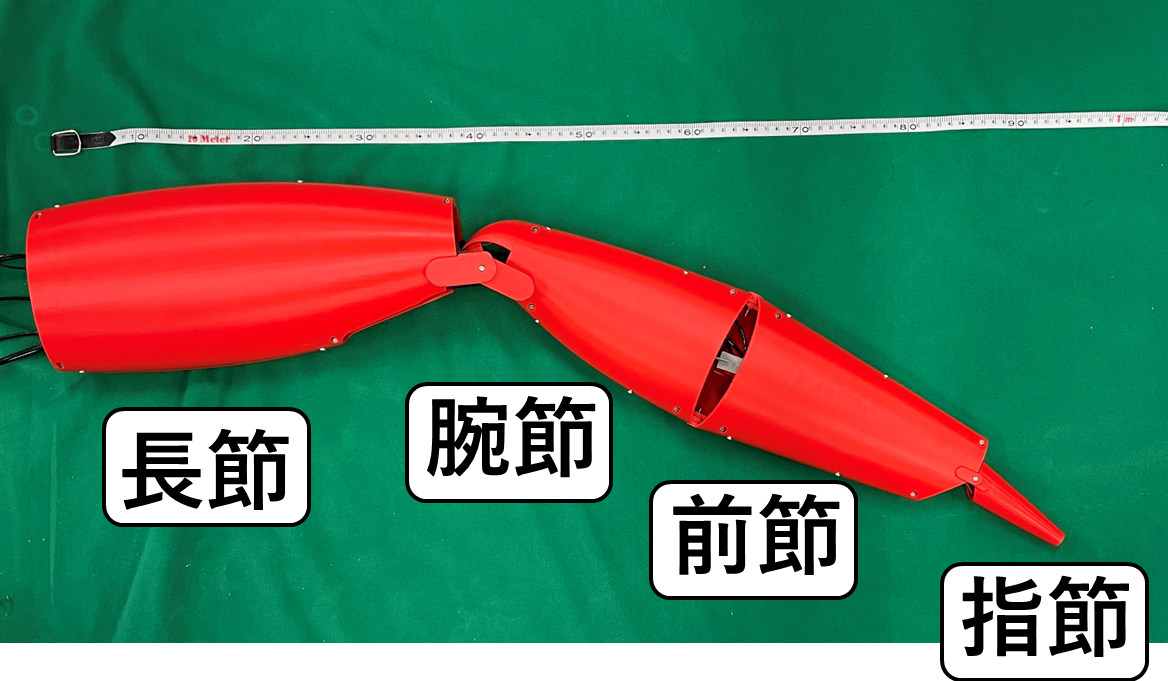
\includegraphics[scale=0.1]{image/jikki_2.png}
    \vspace{-4mm}
    \caption{実機の外観}
    \label{fig:jikki}
  \end{minipage}
  \hspace{0.04\columnwidth}
  \begin{minipage}[b]{0.47\columnwidth}
    \centering
    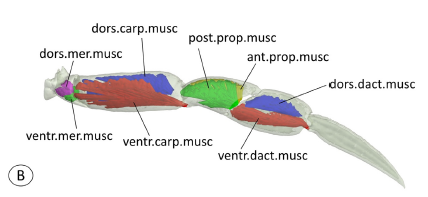
\includegraphics[scale=0.35]{image/crabmuscle_campare.PNG}
    \vspace{-2mm}
    \caption{蟹模倣ロボット\cite{crab}}
    \label{fig:kinhaichi}
  \end{minipage}
\end{figure}
\begin{figure}[t]
  \begin{minipage}[b]{0.47\columnwidth}
    \centering
    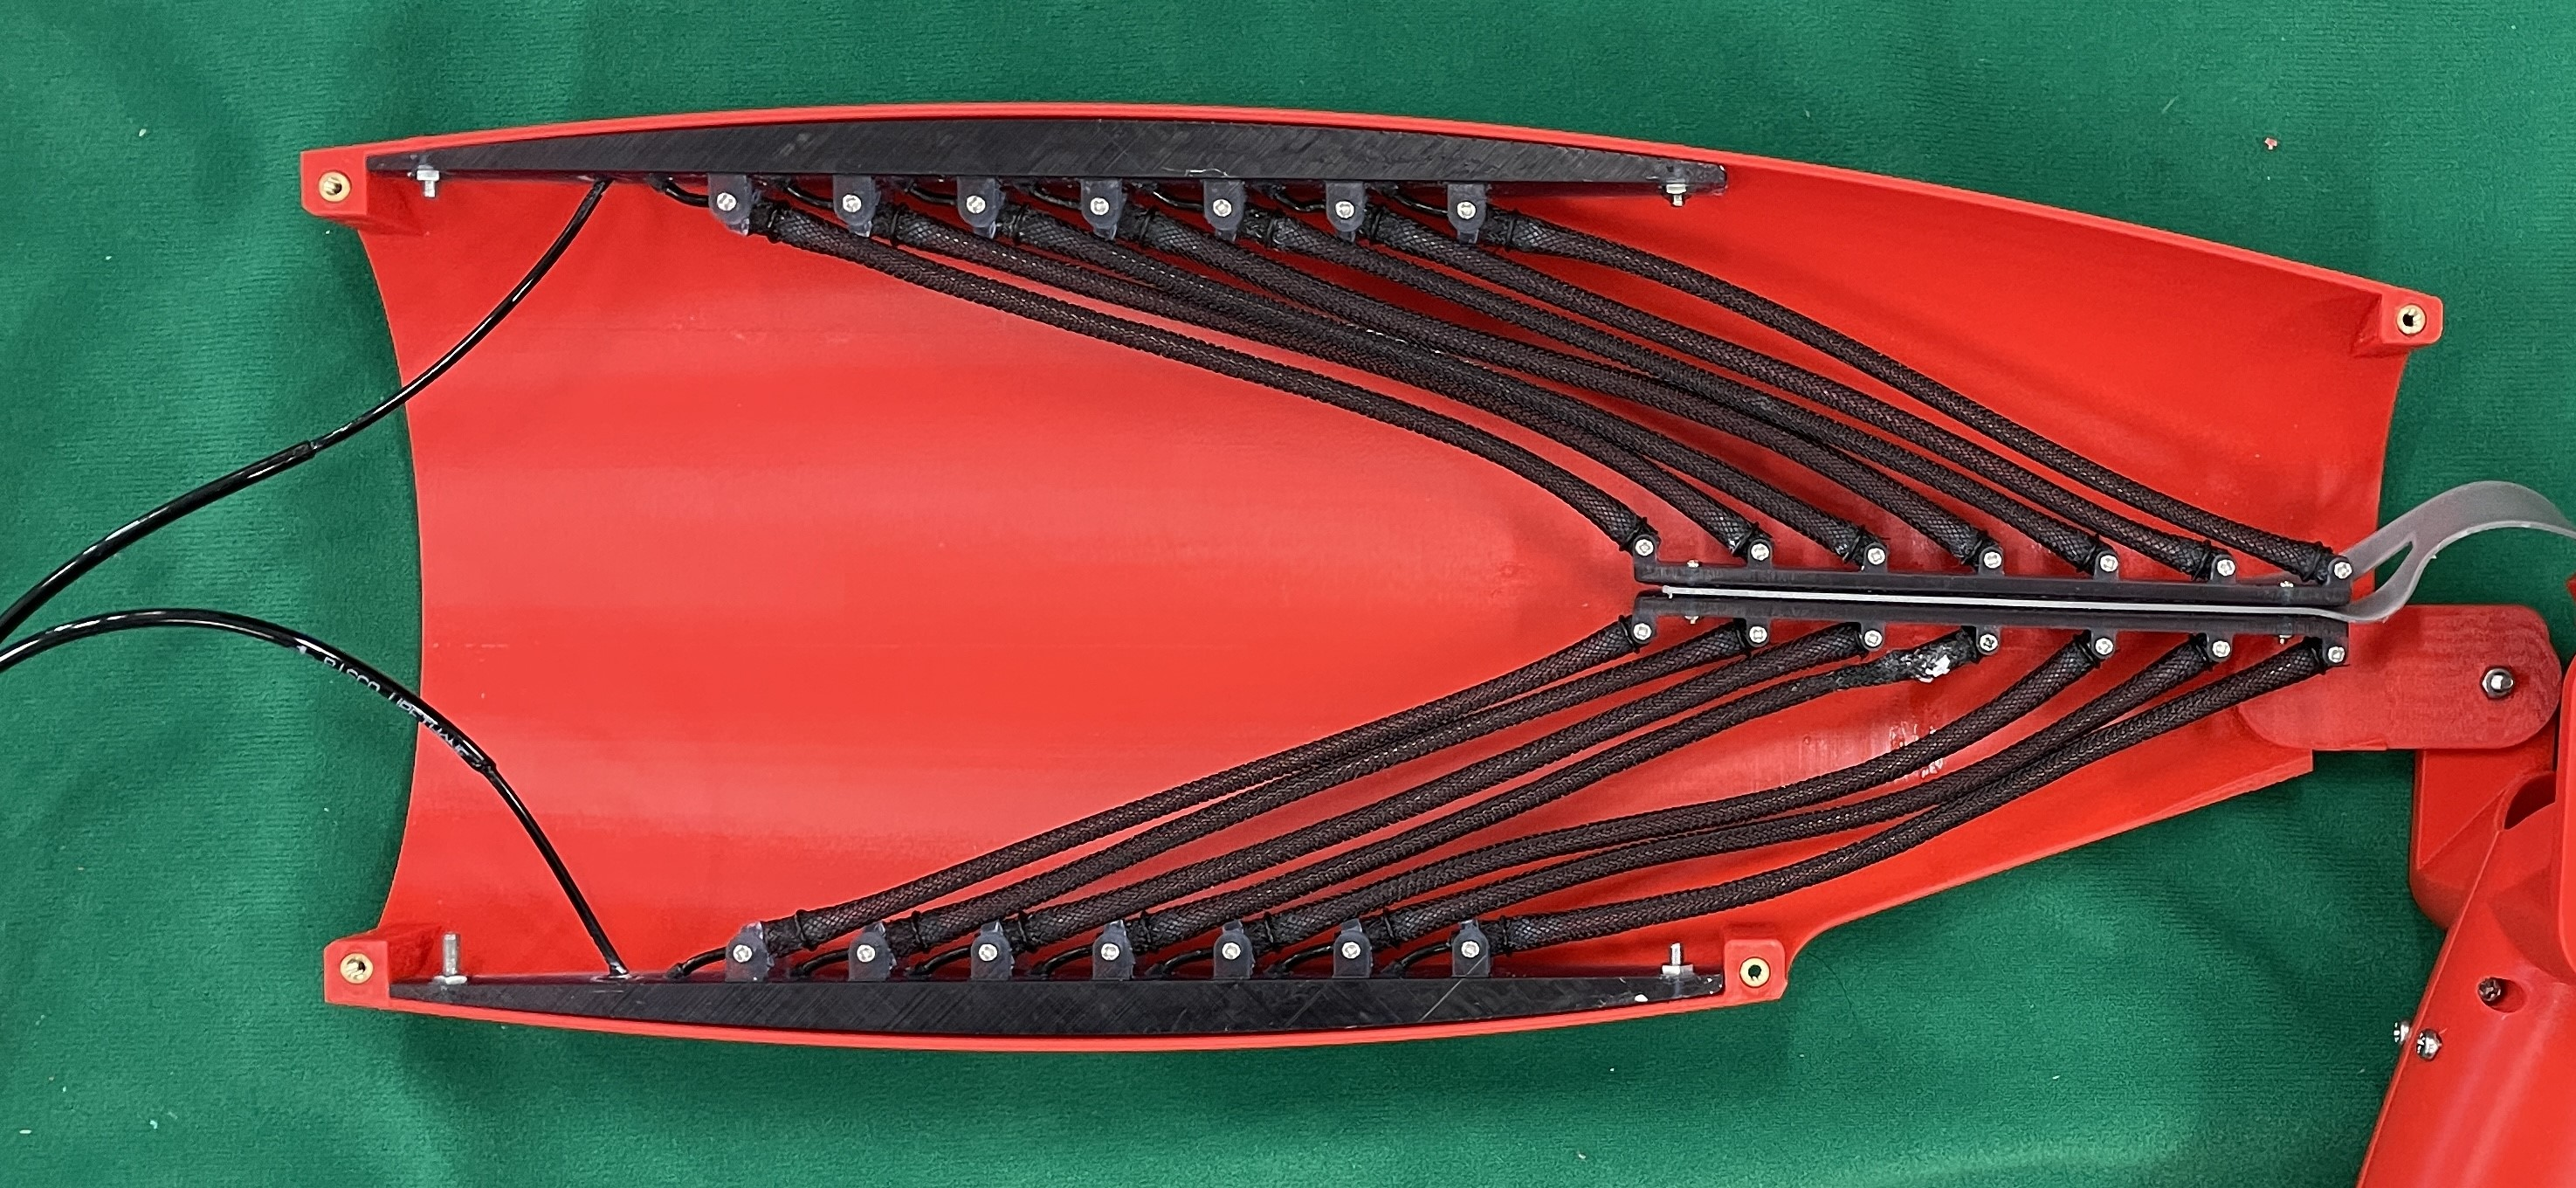
\includegraphics[scale=0.03]{image/crabmuscle.jpg}
    \vspace{2mm}
    \caption{実機内部の筋配置}
    \label{fig:muscle}
  \end{minipage}
  \hspace{0.04\columnwidth}
  \begin{minipage}[b]{0.45\columnwidth}
    \centering
    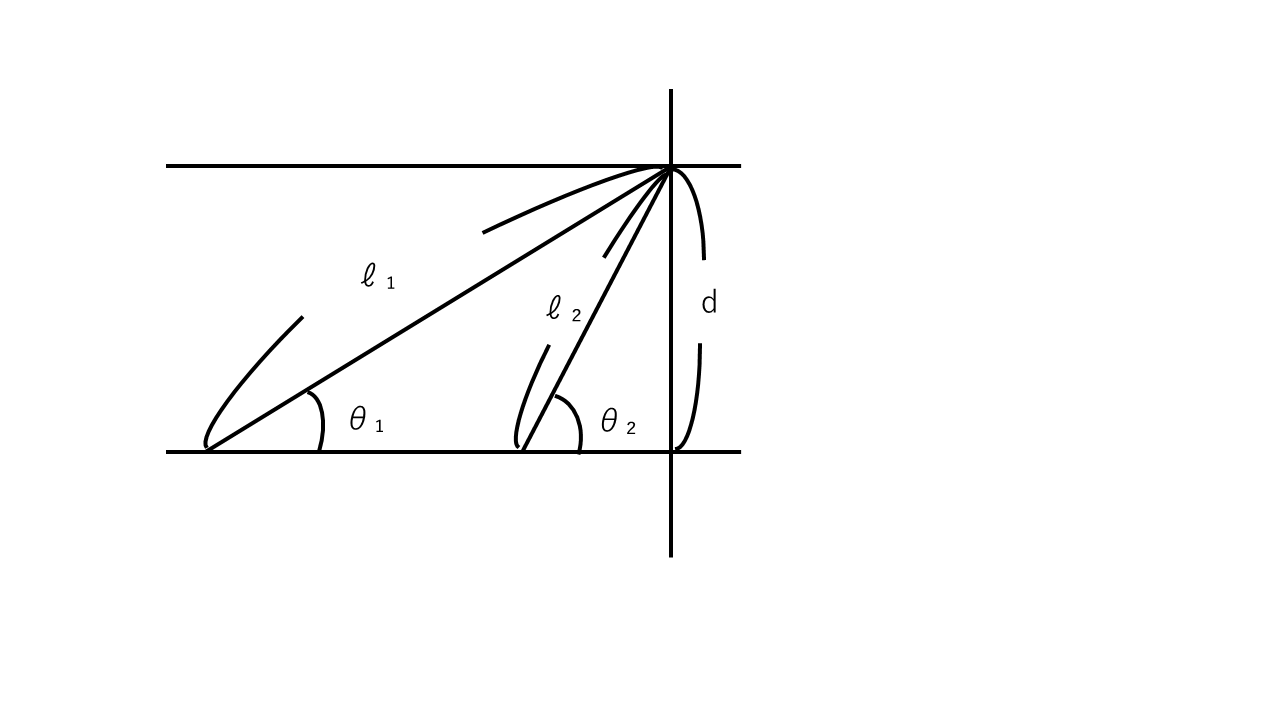
\includegraphics[scale=0.18]{image/keisan_1.png}
    \vspace{-4.5mm}
    \caption{実機の簡易モデル}
    \label{fig:keisan_1}
  \end{minipage}
\end{figure}
%%%%%%%%%%%%%%%%%%%%%%%%%%%%%%%%%%%%%%%%%%%%%%%%%%%%%%%%%%%%%%%%%%%%%%%%%%%%%%%
\vspace*{-4mm}
\begin{figure*}[t]
  \centering
  \subfigure[長節-腕節間の動作実験]{%
  \label{fig:move1} 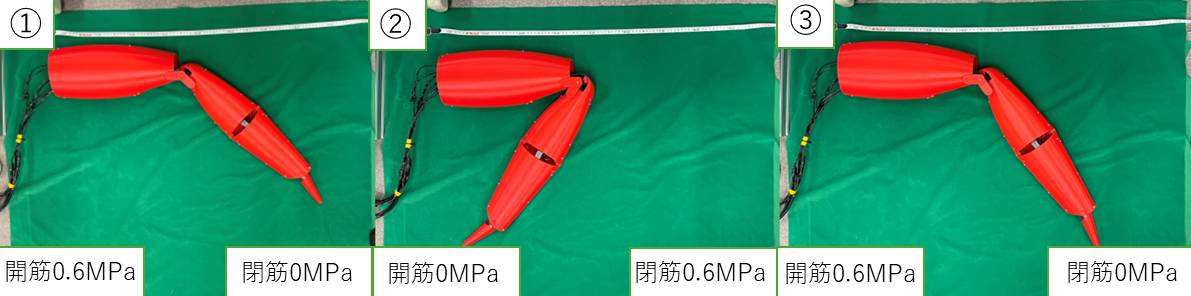
\includegraphics[scale=0.4]{image/chousetu-wansetu.png}}\\%
  \vspace{-2mm}
  \subfigure[腕節‐前節間の動作実験]{%
  \label{fig:move2} 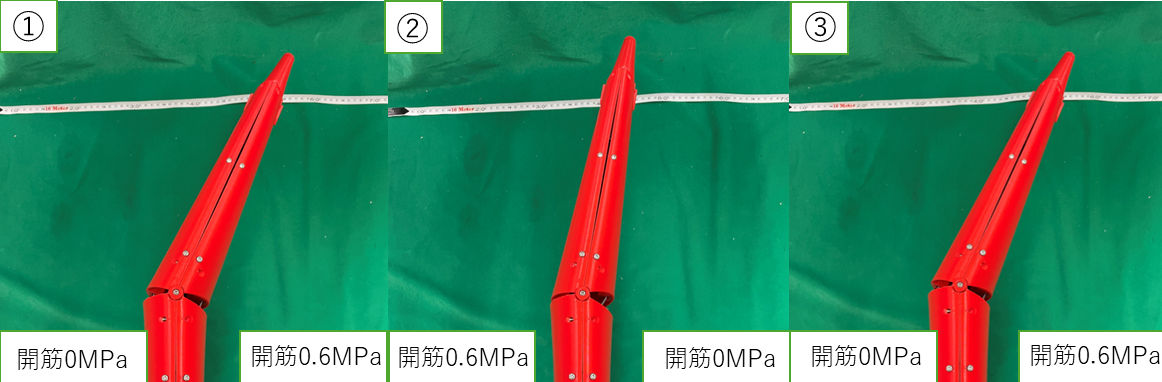
\includegraphics[scale=0.3]{image/wansetu-zensetu.png}}%
  \vspace{-2mm}
  \subfigure[前節‐指節間の動作実験]{%
  \label{fig:move3} 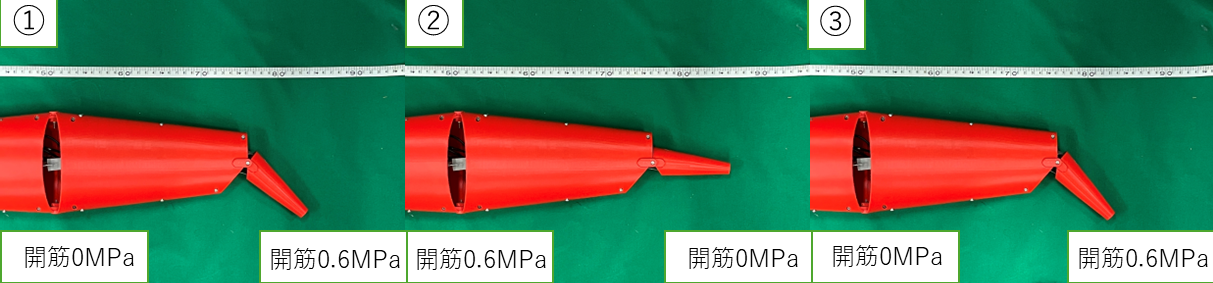
\includegraphics[scale=0.4]{image/zensetu-sisetu.png}}%
  \vspace{-2mm}
  \caption{動作実験の様子.ここで開筋は関節を開く方向に,閉筋は閉じる方向に作用する羽状筋を指す.}
  \label{fig:move}
  \vspace{-2mm}
\end{figure*}
%%%%%%%%%%%%%%%%%%%%%%%%%%%%%%%%%%%%%%%%%%%%%%%%%%%%%%%%%%%%%%%%%%%%%%%%%%%%%%%
\vspace*{-2mm}
\section{結言}

本稿では,外骨格生物模倣ロボットの開発をするにあたって課題となる細径MPA の作成方法と固定方法について改良を行った.
今後は羽状筋の構築,およびカニの歩脚を模したロボットの開発を行い,可動域などについて検証を行う.

%%%%%%%%%%%%%%%%%%%%%%%%%%%%%%%%%%%%%%%%%%%%%%%%%%%%%%%%%%%%%%%%%%%%%%%%%%%%%%%
\begin{thebibliography}{99}
  \bibitem{wakimoto}
  脇本修一,
  細径McKibben型人工筋の開発と用途開拓,
  計測と制御,57巻,11号,pp.812-815,2018
  
  \bibitem{crabrobot1}
  CHEN, Xi, et al. Study on the Design and Experimental Research on a Bionic Crab Robot with Amphibious Multi-Modal Movement, Journal of Marine Science and Engineering,10,12,p.1804,2022
  
  \bibitem{crabrobot2}
  中西大輔,長谷川侑大,浪花啓右,杉本靖博,
  細径空圧筋を用いた羽状筋および外骨格生物模倣ロボットの開発,ロボティクス・メカトロニクス講演会2024,2A1-L08,2024.

  \bibitem{crab}
  D.Hazerli and S.Richter,
  Why“swimming crabs”are able to swim-The importance of the axial skeleton:A comparison between the“swimming crab”Liocarcinus depurator and two other brachyuran crabs (Cancer pagurus, Carcinus maenas) using μCT and 3D-reconstruction,
  Arthropod Structure&Development,
  59,p.100972,2022

 \end{thebibliography}
 %%%%%%%%%%%%%%%%%%%%%%%%%%%%%%%%%%%%%%%%%%%%%%%%%%%%%%%%%%%%%%%%%%%%%%%%%%%%%%%
\end{document}